\subsection{UC3 - Sincronizzazione file da server a client}
\label{UC3}
\begin{figure}[H]
    \centering
    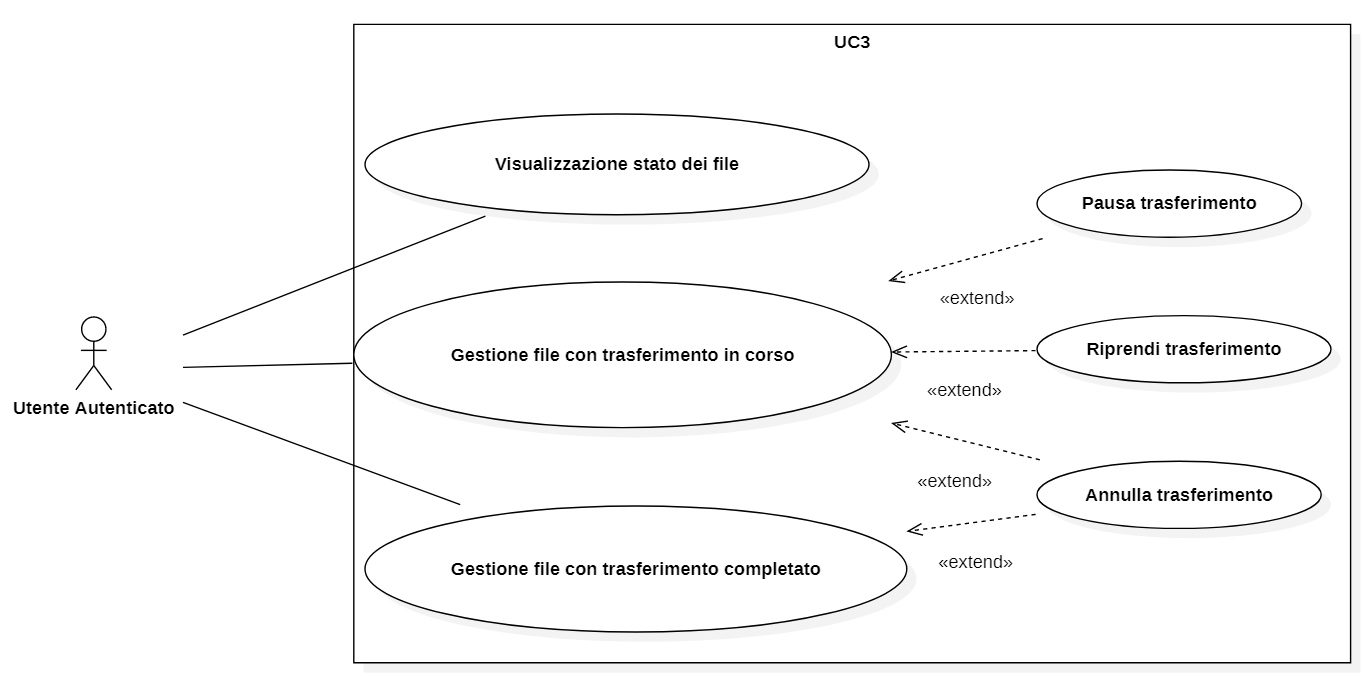
\includegraphics[scale = 0.7]{components/img/UC3.png}
    \caption{UC3 - Sincronizzazione file da server a client}
\end{figure}
\begin{itemize}
\item \textbf{Attore Primario:} Utente autenticato;
\item \textbf{Attore Secondario:} \glo{Zextras Drive};
\item \textbf{Precondizione:} L'utente ha necessità di sincronizzare uno o più file presenti sul server verso il client;
\item \textbf{Postcondizione:} L'utente ha sincronizzato i file dal server al client;
\item \textbf{Scenario principale:}
    \begin{enumerate}
    \item L'utente vuole sincronizzare dei file dal server al client;
    \item Viene scelto l'insieme dei file che dovrà essere sincronizzato;
    \item La sincronizzazione delle modifiche viene attivata per l'insieme scelto.
    \end{enumerate}
\item \textbf{Estensioni:}
    \begin{itemize}
    \item Visualizza messaggio di errore di rete (UC7 \S{}\ref{UC7});
    \item Visualizza messaggio di errore spazio non disponibile in locale (UC10 \S{}\ref{UC10});
    \item Visualizza messaggio di opzione per il file in conflitto (UC15 \S{}\ref{UC15}).
\end{itemize}
\end{itemize}
